\section{研究并联电路}\label{sec:8-13}

在 “\hyperref[sec:8-2]{用安培表测电流强度}” 和 “\hyperref[sec:8-4]{用伏特表测电压}” 的实验里,
我们已经知道:

\textbf{并联电路中的总电流强度等于各支路中的电流强度之和};

\textbf{并联电路中,各支路两端的电压都相等}。

\begin{wrapfigure}[12]{r}{7cm}
    \centering
    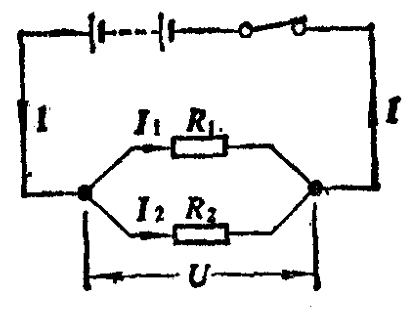
\includegraphics[width=6cm]{../pic/czwl2-ch8-33}
    \caption{}\label{fig:8-33}
\end{wrapfigure}

\begin{enhancedline}
现在我们来研究整个并联电路的总电阻跟各支路的电阻的关系。
跟上节一样,我们也是利用欧姆定律来解决这个问题。
设并联电路的总电阻为 $R$,各支路的电阻分别为 $R_1$ 和 $R_2$(图 \ref{fig:8-33})。
那么,由于
$$ I = \dfrac{U}{R}\,\text{,} I_1 = \dfrac{U}{R_1}\,\text{,} I_2 = \dfrac{U}{R_2}\,\juhao $$

把上列各式代入 $I = I_1 + I_2$ 中, 就得到
$$ \dfrac{U}{R} = \dfrac{U}{R_1} + \dfrac{U}{R_2} \,\text{,} $$
所以, $\dfrac{1}{R} = \dfrac{1}{R_1} + \dfrac{1}{R_2}$。
这表明\textbf{并联电路的总电阻的倒数,等于各并联导体的电阻的倒数之和}。

从实验知道,几个导体并联起来,总电阻比任何一个导体的电阻都小。
这是因为导体并联起来就相当于增大了导体的横截面积。

并联是把各种用电器连接在电路里的主要方法。
例如,接在照明电路里的电灯、收音机、电视机、电风扇等用电器,就是并联着的,它们的电压都是 220 伏特。


\liti 将两个阻值分别为 12 欧姆和 60 欧姆的电阻并联起来,求并联后的总电阻。

解:$\begin{aligned}[t]
    &\text{把题目给的数据代入公式} \dfrac{1}{R} = \dfrac{1}{R_1} + \dfrac{1}{R_2} \;\text{,} \\
    &\dfrac{1}{R} = \dfrac{1}{12\oumu} + \dfrac{1}{60\oumu} = \dfrac{6}{60\oumu} \;\text{,} \\
    &R = \dfrac{60\oumu}{6} = 10\oumu \;\juhao
\end{aligned}$

答:并联后的总电阻是 10 欧姆。



\liti 在图 \ref{fig:8-34} 所示的电路中,电源的电压是 36 伏特,
灯泡 $L_1$ 的电阻是 10 欧姆,$L_2$ 的电阻是 40 欧姆。
求 $K_1$、$K_2$ 都闭合时,电路的总电阻和干路里的电流强度。

\begin{wrapfigure}[6]{r}{7cm}
    \centering
    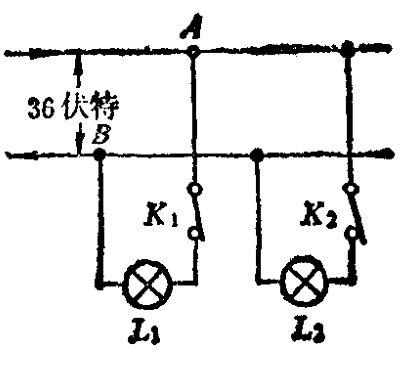
\includegraphics[width=6cm]{../pic/czwl2-ch8-34}
    \caption{}\label{fig:8-34}
\end{wrapfigure}

首先要认清灯泡 $L_1$ 和 $L_2$ 是并联的。
我们可以先求出总电阻,再求干路里的电流强度;
也可以先求各支路里的电流强度,再求干路里的电流强度和总电阻。
这里用前一种方法来解,后一种方法同学们自己做,看看结果是否相同。

解:$\begin{aligned}[t]
    &\dfrac{1}{R} = \dfrac{1}{R_1} + \dfrac{1}{R_2} = \dfrac{1}{10\oumu} + \dfrac{1}{40\oumu} = \dfrac{5}{40\oumu}\;\text{,} \\
    &R = \dfrac{40\oumu}{5} = 8\oumu \;\juhao \\
    &I = \dfrac{U}{R} = \dfrac{36\fute}{8\oumu} = 4.5\anpei \;\juhao
\end{aligned}$

答:电路里的总电阻是 8 欧姆,干路里的电流强度是 4.5 安培。
\end{enhancedline}

不少物理题有一种以上的解法。所以,在解出一道物理题之后,要想想还有没有别的解法,如果有,用所想出来的解法试试。
这样可以提高你们灵活运用知识的能力。


\lianxi

(1) 一根铜导线和一根镍铬合金线,长短粗细都相等,把它们并联在电路里,
那根导线里的电流大?哪根导线两端的电压大?为什么?

(2) 有人说:“并联的几个导体的总电阻,等于各导体的电阻的倒数之和。”
这个说法对吗?如果不对,错在哪里?

\begin{wrapfigure}[10]{r}{7cm}
    \centering
    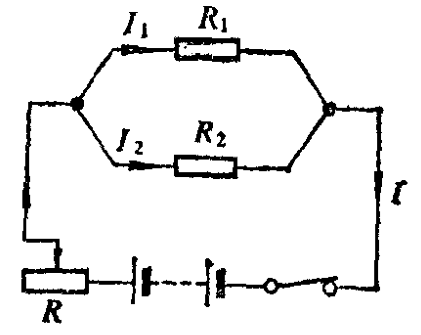
\includegraphics[width=6cm]{../pic/czwl2-ch8-35}
    \caption{}\label{fig:8-35}
\end{wrapfigure}

(3) 求 2 欧姆的电阻和 6 欧姆的电阻并联后的总电阻。

(4) 把上题中的两个电阻并联。如果 2 欧电阻上的电压是 6 伏特,那么,
每个电阻里的电流强度和并联部分的总电流强度各是多大?

(5) 修理仪表时,要 5 千欧电阻和 20 千欧电阻各一只,但手边只有几只 10 千欧的电阻。
想想看,能不能利用这些 10 千欧的电阻来解决问题?怎样解决?

(6) 在图 \ref{fig:8-35} 所示的电路中,电源是 6 伏特的蓄电池组,$R_1 = 20$ 欧姆, $R_2 = 10$ 欧姆,
$I_1 = 0.2$ 安培。求 $I_2$ 和 $I$。

(7) 有一个电阻值已看不清楚的电阻器 $R_1$, 我们想要测出它的电阻值,
手边只有一个电池组、一个安培表、一个电阻值看得清楚的电阻器 $R_2$ 和几根导线。
你有办法测出 $R_1$ 的电阻值吗?说出你的办法和理由。

